In this section, we elucidate our methodology and approaches concerning the various machine learning models 
that we have developed for the Bomberman game agent. We will also substantiate what has proven effective, articulate 
the concepts we have discarded, and expound upon the rationale for ultimately selecting the model we have submitted.

\subsection{Our final best model (first project)}

Explained by Berkay

\subsection{Our second best model (second project)}

In our quest to develop our second best model for Bomberman, we embarked on a journey where we collected data pairs of game 
states and rule-based agent actions. Using this data, we trained a machine learning model, optimizing it to mimic 
the rule-based agent's decision-making. The AI, powered by a carefully chosen model architecture and loss function, 
should learn to imitate the agent's actions in various game states. This approach allowed us to create an AI actor 
that could navigate Bomberman's challenges and make decisions based on the learned rules and actions of the rule-based agent.

To enhance our model and surpass the rule-based agent's performance we want to use deep Q-learning. We extended our actor-critic architecture by 
introducing a critic network to estimate Q-values, allowing the agent to understand the long-term consequences of its actions. 
We implemented an exploration strategy, such as epsilon-greedy, to encourage the model to explore new strategies and avoid getting 
stuck in suboptimal actions. Lastly, we employed a reward shaping mechanism that provided tailored rewards for encouraging desirable behaviors.

The basic idea is as follows: we first pretrain a model that imitates the rule-based agent and then further improve this model using deep Q-learning. 
However, the deep Q-learning part is not explained in detail in this section since the architecture is almost identical to what was explained in the 
section about our final project. Nevertheless, we do discuss where there were changes, such as in the features.

We chose PyTorch as our primary library because it offers a flexible and dynamic computation graph, allowing us to easily design and 
experiment with complex neural network architectures. Additionally, its extensive community support, rich ecosystem of pre-built modules, 
and integration with GPU acceleration make it an ideal choice for achieving our goals efficiently.

\subsubsection*{Data Collection}

In our data collection process, we began by generating extensive game data through multiple playthroughs of Bomberman with 
our rule-based agent. During these sessions, we recorded both the game states and the corresponding actions taken by the agent, 
encompassing movements (left, right, up, down) and bomb placements.

The code below explains how we implemented it. First, we create a ReplayBuffer from the rule-based agent 
to record how the rule-based agent played. The buffer returns a tuple containing the list of states and actions 
taken by the rule-based agent when \verb|get| is called. The actions are one-hot encoded so that they can later be used as 
classes during network training. In \verb|setup_training|, the \verb|RuleBased_Replay| is initialized, where \verb|capacity| determines 
how many games we want to store, typically ranging from 500,000 to 1,000,000 games. In \verb|game_events_occurred|, 
we store each state along with the corresponding action taken by the rule-based agent because we have the 
rule-based agent play only for training purposes in \verb|callback.py|.

\begin{lstlisting}[language=Python]
    
    ...

    from collections import namedtuple, deque

    ...

    class RuleBased_Replay():
        def __init__(self, capacity):
            self.states = deque([], maxlen=capacity)
            self.one_hot_labels = deque([], maxlen=capacity)

        def push(self, state, action):
            self.states.append(state)

            # convert action to one-hot
            a = [0,0,0,0,0,0]
            a[action] = 1
            self.one_hot_labels.append(a)

        def get(self):
            return self.one_hot_labels, self.states

        def __len__(self):
            return len(self.one_hot_labels)
        
    ...

    def setup_training(self):

    ...

        self.rule_based_replay = RuleBased_Replay(capacity=MEMORY_BUFFER)
    
    ...

    def game_events_occurred(self, old_game_state: dict, self_action: str, new_game_state: dict, events: List[str]):
        self.rule_based_replay.push(
            state_to_features(old_game_state), 
            ACTIONS.index(self_action))
        
        ...
    
    ...
    
\end{lstlisting}

Once we amassed a substantial dataset, we transformed it into a format compatible with PyTorch's Dataset class. 
Each dataset entry consisted of two fundamental components: the game state and the associated action label. We represented 
the game states as tensors to ensure seamless integration with PyTorch.

\begin{lstlisting}[language=Python]
    ...

    train_ds = CTDataset(data, labels)

    ...

\end{lstlisting}

Leveraging PyTorch's Dataset class, we crafted a custom dataset equipped with efficient data loading and preprocessing capabilities. 
During training, we harnessed PyTorch's DataLoader to batch and load the data conveniently. 
Depending on the problem at hand, we also applied data augmentation techniques, such as random rotations or flips, 
to enhance the diversity of our training samples and boost the model's generalization capabilities.

\begin{lstlisting}[language=Python]
    ...

    train_dl = DataLoader(train_ds, batch_size=batch_size, shuffle=True)

    ...
    
\end{lstlisting}

To facilitate model training and evaluation, we divided the dataset into distinct sets for training, validation, 
and testing purposes. This partitioning allowed us to gauge our model's performance on unseen data and make necessary adjustments.

\subsubsection*{State Representation}

\begin{figure}[tb]
    \centering
    \subfloat[\label{fig:autoencoder}]{%
      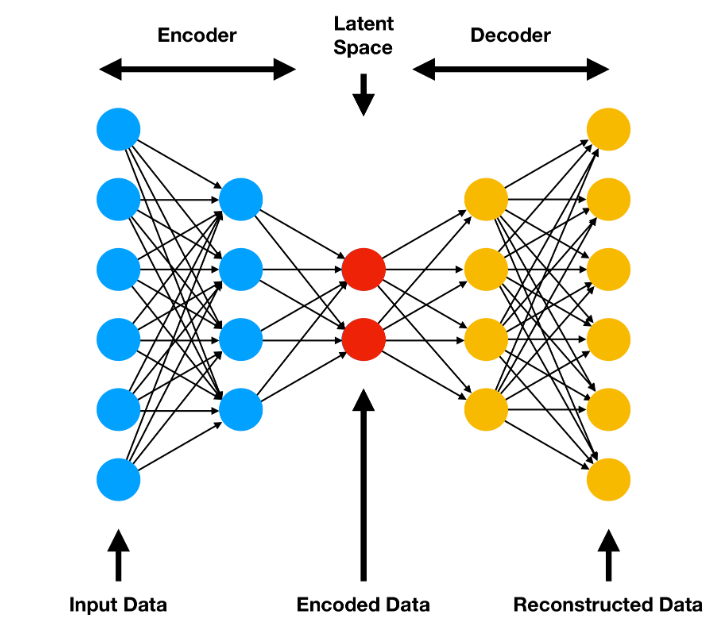
\includegraphics[width=\twoImgWidth]{images/autoencoder}%
    }%
    \hfill%
    \subfloat[\label{fig:sparseMatrix}]{%
      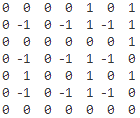
\includegraphics[width=\twoImgWidth]{images/sparse_matrix_game}%
    }%
    \captionadjust%
    \caption{\label{fig:autoencoderSparseMatrix}
    \protect\subref*{fig:autoencoder}: Example of an autoencoder network \cite{Img:autoencoder}.
    \protect\subref*{fig:sparseMatrix}: The 7x7 game state is getting more and more sparse over time.
    }%
\end{figure}

In our past work on Bomberman, we recognized the critical importance of state representation in optimizing the performance 
of our AI agents. Specifically, we focused on the transition from the original 17x17 grid, which encompassed the entire Bomberman field, 
to a reduced 7x7 grid. To accomplish this, we centered the agent's viewpoint in the 17x17 grid to capture the immediate surroundings. 
This reduction was not just a matter of simplification, it is especially important to prevent overfitting. When the agent network consistently 
receives the entire 17x17 field for learning, there's a high likelihood that the network will memorize training patterns and struggle with test data. 
The objective is to ensure that the agent learns the intelligent strategies of the rule-based agent to a certain extent, at the very least, mastering how 
to play the game effectively without necessarily striving for extreme efficiency. In doing so, we also took inspiration from humans who, like our AI, do not perceive 
the entire field but rather focus on a specific part while filtering out the rest.
Reducing the field to 7x7 retained key spatial relationships 
and relevant game features while simplifying the representation, thus allowing our AI agents to focus on essential information.
To determine if there is a difference in how the rule-based agent plays the game when the view box is reduced to 7x7, we had the following idea:
lets consider the following function: 
\begin{equation} \label{eq:1}
G_A(f,v) \rightarrow \{\text{up, down, left, right, bomb}\}
\end{equation}

that outputs the best possible action the agent could do. The field is described by $f$ and $v$ is the viewbox of the agent. We did many 
test rounds with the rulbased agent on an 17x17 field with \verb|--seed 1| for a comparable result. We had two scenarios
in one scenario the rulbased agent saw the whole 17x17 field e.g $G_a(f, 17\times17)$, on the other scenario the agent saw a
7x7 field e.g $G_a(f, 7\times7)$. Then we calculated the probability $p$ to find out how likely it is, that the actions in both scenarios are different in one step.
We simply counted the number of different actions and divided them by the maximum number of steps.
For the 7x7 field we had a probability of $p=0.054$ which was the best value for us compared to a 5x5 or 3x3 viewbox.\\

But, please note that initially, we interpreted this number $p$ quite differently. The probability distribution is not uniform. 
It turns out that the agent with a 7x7 viewbox makes more diverse actions as the game progresses compared to the agent with a 17x17 viewbox. 
This happens because towards the end of the game, there are fewer items or opponents within the 7x7 view, and the agent becomes uncertain about its actions. 
A better approach would be to determine the probability distribution function $p(X = k)$, where $k$ represents the number of steps in a game.
For example lets look at the probability at the beginning of the game $p(0 \geq X \leq 20) = 0$ and at the end of the game $p(310 \geq X \leq 330) = 0.47$
We had to come up with a solution to address this issue. Once the 7x7 field was empty of items or opponents, the agent switched to an exploration mode and randomly 
searched the surroundings for potential objectives.\\

However, the 7x7 field often contained sparse feature data see \autoref{fig:sparseMatrix}, with many cells remaining empty or irrelevant. 
To efficiently handle this challenge, we employed an encoder-decoder network see \autoref{fig:autoencoder}. This architecture allowed us 
to compress the sparse feature data effectively. But before we delve into how the encoder-decoder network functions, we need to address how our 
features are generated within the \verb|state_to_features| function. First, we restrict the agent's field of view to 7x7. Then, we create a 7x7 map 
with the agent in the center, represented by the number 100. Here, 0 denotes open space, 1 represents crates, -1 signifies walls, 5 indicates coins, 15 represents 
opponents, and 25 stands for bombs. Another 7x7 map contains the hidden features, which are features that would otherwise overlap with those on the first map. 
These hidden features include whether all agents can ignite a bomb, represented as 0 or 1. A third map with hidden features describes the blast radius of a 
bomb along with its respective countdown. These three 7x7 maps, also known as channels, are then merged into a 
single 147-element array. Below is a code snippet:

\begin{lstlisting}[language=Python]
    ...

    def state_to_features(game_state: dict) -> np.array:
        field = game_state["field"]
        bombs = game_state["bombs"]
        explosion_map = game_state["explosion_map"]
        coins = game_state["coins"]
        agent = game_state["self"]
        others = game_state["others"]

        my_pos = make_field(agent[3])

        ...

        # non hidden features
        # make_field create a matrix from coordinate list
        channel1 = make_field(bombs) + make_field(others) + make_field(coins) 
                                     + field + my_pos

        # can agent put a bomb
        channel2 = extract_bom_is_possible_to_field(others) +  
                   extract_bom_is_possible_to_field(agent)

        channel3 = make_real_explosion_map(bombs, explosion_map)

        ...

        vf = make_viewbox(7,7, [channel1, channel2, channel3])
        return vf.flatten()

    ...
    
\end{lstlisting}

Next, we want to modify the \verb|state_to_features| function to further compress the data in the 149-element array while preserving as much information as possible. 
To achieve this, we'll utilize an encoder-decoder network see \autoref{fig:autoencoder}. This network has the same output dimension as the 
input dimension and aims to reconstruct the 
input data. However, in the dense layers, the features are reduced up to a certain point (encoded data layer). Then, in subsequent dense layers, the 
features are expanded back to the input dimension. If the network can effectively reconstruct the input data, we'll use it and extract the encoded data layer, 
which we will return in the \verb|state_to_features| function. We were able to compress the data from the 149-element array to a 72-element array. These data will 
now be used for our second network to train the rule-based agent. Details about both networks will be explained later 
in Model Architecture. Here's the modification of the \verb|state_to_features| function once again:

\begin{lstlisting}[language=Python]
    ...

    def state_to_features(game_state: dict) -> np.array:

        ...

        vf = make_viewbox(7,7, [channel1, channel2, channel3])
        compressed_features = encoder_decoder_network.encode(vf.flatten(), 72)
        return compressed_features

    ...

\end{lstlisting}

The encoder module was instrumental in feature learning, condensing the sparse data to capture essential features efficiently. 
Additionally, it reduced dimensionality, enhancing computational efficiency and reducing noise in the data. During decoding, the network could 
reconstruct the original 7x7 state representation from the compressed data, ensuring that no critical information was lost in the process.

\subsubsection*{Model Architecture}

\begin{figure}[H]
    \centering
    
    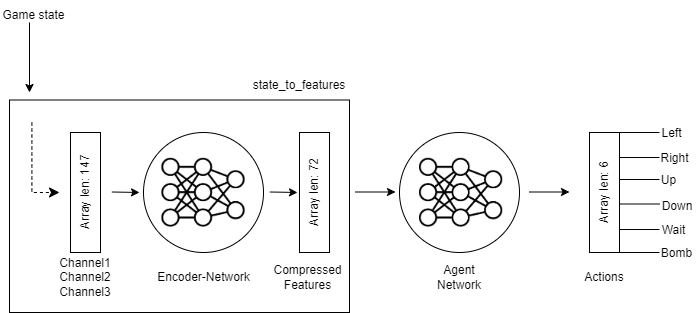
\includegraphics[width=\oneImgWidth]{images/network-arch}%
    
    \captionadjust%
    \caption{\label{fig:network-arch} Here is how our two models come into play.
    }%
\end{figure}

In total, we employ two neural networks see \autoref{fig:network-arch}. The encoder network is utilized within the \verb|state_to_features| function to compress the 
generated features, as they contain many repetitive entries, such as 0, 1, or -1. Through this compression, our aim is not only to reduce 
the data size but also to create patterns that make it easier to describe a state. This is particularly significant for the second network. 
The second network is the agent network, which receives data from the \verb|state_to_features| function and endeavors to predict the best action.
Here are the characteristics of the two networks listed:

\begin{verbatim}
Encoder Network:
    Layers: 1 Inupt, 5 Hidden, 1 Output
    Neurons: 
        Input1: 147, Hidden1: 124, Hidden2: 102, Hidden3: 72,
        Hidden4: 102, Hidden5: 124, Output1: 147

Agent Network:
    Layers: 1 Inupt, 3 Hidden, 1 Output
        Neurons: 
            Input1: 72, Hidden1: 64, Hidden2: 32, Hidden3: 16, Output1: 6
\end{verbatim}

\subsubsection*{Loss function and optimizer}

We have two models: the encoder network for further feature compression and the agent network, which is tasked with 
learning how to play the game effectively. Additionally, the agent is initially meant to imitate the rule-based agent, which is 
achieved through classification. Later on, the agent will be further improved using deep Q-learning. For all these scenarios, we require 
different loss functions and optimizers with varying learning rates because there are more suitable optimizers and loss functions for specific cases.\\

For the encoder network, the ADAM optimizer with a learning rate of $0.001$ proved to be the most effective, and the chosen loss 
function was the MSE (Mean Squared Error) loss. During experimentation, we observed that the loss function did not converge to near 
zero with a learning rate of $>0.001$, and with a learning rate of $<0.001$, it converged towards zero, albeit very slowly. \\

For the agent network when mimic the rulbased agent, we used the ADAM optimizer with a learning rate of $0.0001$ and the Cross-Entropy loss function because
in classification, the goal is to assign probabilities to each class. Cross-entropy loss directly deals with probability 
distributions and can handle multi-class problems efficiently.\\

For the agent network during deep Q-learning, we used the ADAM optimizer with a learning rate of $0.0001$ and the Huber loss as the loss function.
It is designed to balance the benefits of mean squared error (MSE) and mean absolute error (MAE) loss functions.
But for any reason was the MSE loss better for the encoder network than the Huber loss.

\subsection{Other aproaches that we had}

At the beginning of the project, we had several other ideas about how to construct our AI agent. One alternative idea was to use Q-tables. 
For the coin collector agent, we considered the concept that it would only perceive one coin, specifically the one closest to it.
However, in the end, we discarded all of these ideas, and the following reasons explain why:

\subsubsection{Q-Tables}

Q-tables (Quality or Q-value tables) are used to approximate and store the expected cumulative rewards (Q-values) associated 
with different state-action pairs in a Markov Decision Process (MDP).
Rows represent states or state descriptions, columns represent possible actions that can be taken in those states.
Each cell in the table stores the expected cumulative reward, denoted as Q-value, for taking a specific action in a specific state.

The Q-value for a state-action pair $(s, a)$ represents the expected sum of rewards an agent can achieve by taking 
action $a$ in state $s$ and following a specific policy thereafter. The Q-value is typically updated iteratively as the 
agent explores and learns from its interactions with the environment.
Once the Q-table has converged or reached a sufficiently accurate representation of the optimal Q-values, 
the agent can select actions that maximize these Q-values

The equation for updating the Q-table in the context of Q-learning is as follows:
\begin{equation} \label{eq:1}
Q(s, a) = (1 - \alpha) \cdot Q(s, a) + \alpha \cdot [R(s, a) + \gamma \cdot \max_a Q(s', a)]
\end{equation}

In this equation:

\begin{itemize}

\item $Q(s, a)$ represents the Q-value for a specific state-action pair (s, a).
\item $\alpha$ (alpha) is the learning rate, determining the weight given to the new information when updating the Q-value. It's a value between 0 and 1.
\item $R(s, a)$ is the immediate reward received after taking action 'a' in state 's'.
\item $\gamma$ (gamma) is the discount factor, which controls the importance of future rewards. It's also a value between 0 and 1.
\item $Q(s', a)$ represents the Q-value of the next state 's' after taking action 'a', and \(a\) is the action that maximizes this Q-value.

\end{itemize}

The rason why we discarded this idea is that the bomberman environment has a large number of states, even when using a reduced state representation. 
Each cell on the game board can have multiple attributes (e.g., walls, crates, coins, enemies, bombs), resulting in an extensive state space. 
Creating a Q-table to store Q-values for every state-action pair in such a high-dimensional space would be impractical.


\subsubsection{Coin-Collector Agent that sees only one coin}

Our coin collector agent was given the entire 17x17 field but only focused on the nearest coin, which was simply added to the \verb|game_state["field"]|. 
It received rewards only when collecting this specific coin. This approach worked very well for us, and the agent could consistently collect nearly 
all the coins later in the game. The advantage of this method is that it doesn't matter how many coins are on the field; the agent doesn't need to be 
retrained. However, for an agent tasked with more complex actions like defeating enemies, destroying crates, and collecting bombs, we couldn't 
pursue this idea. This is because we explored other concepts to enable the agent to perform various tasks effectively, and these concepts are described in this report.